\paragraph{Ziel} In diesem Versuch soll ein Helium-Neon-Laser (im Weiterem HeNe-Laser genannt) untersucht 
werden. Dazu soll der Laser justiert und zum lasen gebracht werden. Danach soll der maximale Resonatorabstand, 
die Polarisation des Laserlichtes, die Wellenlänge und mindestens zwei TEM-Moden vermessen werden. Zusätzlich 
sollen drei Frequenzspektren gemessen werden, die aufgrund der verschiedenen Moden die im Resonator auftreten. 

\section{Theorie}
\label{sec:Theorie}

\paragraph{HeNe-Laser} 
Das besondere an einem Laser ist, dass er monochromatisches Licht mit großer Kohärenz und Intensität aussendet. 
Ein Laser besteht wesentlich aus drei Komponenten einem aktiven Lasermedium, einer Pumpquelle und einem 
Resonator. Der Resonator erzeugt eine optische Rückkopplung und schickt das emittierte Licht so 
zurück auf das Lasermedium. Dadurch entsteht ein selbstanregender Oszillator. Das Lasermedium bestimmt 
das Spektrum das emittiert werden kann. 
\newline
Der HeNe-Laser besteht grundlegend aus einem Laserrohr in dem ein Gasgemisch aus He- und Ne-Atomen im 
Verhältnis 5:1 mit einem Druck von ca. \SI{1.3}{\milli\bar} eingeschlossen ist. Das Laserrohr 
ist mit einem Brewsterfenster abgeschlossen. Ein Brewsterfenster ist ein optisches Gerät welches 
im Brewsterwinkel zur optischen Achse des einfallenden Strahls steht und somit den senkrecht-polarisierten 
Teil des Lichtes teilweise reflektiert, während der parallel-polarisierte Teil ohne Reflexion passiert. 
Folglich tritt nur das parallel-polarisierte Licht ohne Abschwächung aus. In diesem Lasersystem wird 
Neon als Lasermaterial und Helium als Pumpgas bezeichnet. 
Durch elektrische Entladung kann eine Besetzungsinversion im Gasgemisch erzeugt werden. 
Das geschieht in dem das Helium in einen metastabielen Zustand angeregt wird und durch Stöße zweiter Art 
die Anregungsenergie auf die Neon-Atome überträgt. Der Stoß zweiter Art lässt sich wie folgt beschreiben 
\begin{equation*}
A^* + B \rightarrow A + B^* + \Delta E	\; ,
\end{equation*}
dabei bezeichnen $A$ und $B$ Atome im Grundzustand, der Index * bezeichnet dabei den angeregten Zustand des 
jeweiligen Atoms und $\Delta E$ bezeichnet die Energiedifferenz der zwei Energie-Niveaus. Es kommt also 
zum Stoß zweier Atome, eines im angeregten und eines im Grundzustand, als Folge wird das Atom im Grundzustand 
angeregt und das andere Atom wird abgeregt und zusätzlich wird die überschüssige Energie $\Delta E$ frei.
Beim HeNe-Laser können mehrere Linien beobachtet werden, die rote Linie mit Wellenlänge 
$\lambda = \SI{632.8}{\nano\meter}$ ist darunter die intensivste. 

\paragraph{Inversion, Emission, Absorption}
Ziel des Lasers ist die Manipulation des Lasermediums, sodass eine Verstärkung des einfallenden Lichtes auftritt. 
Der einfachste Fall ist dafür in \autoref{fig:sl} dargestellt, darin gibt es zwei mögliche Zustände mit 
Besetzungszahlen $n_1$ und $n_2$ (Grundzustand \& angeregt). Besitzt ein einfallendes Photon 
die Energie des Überganges, kann es absorbiert werden und das Atom ist im angeregten Zustand. Das 
Atom kann nun spontan in den Grundzustand übergehen in dem es ein Photon aussendet, dieser Prozess wird 
spontane Emission genannt. Der Prozess kann aber auch eingeleitet werden, indem ein weiteres Photon 
eingestrahlt wird. Folglich werden zwei Photonen emittiert, beide besitzen die selbe Ausbreitungsrichtung, 
Phase und Energie, dieser Prozess wird induzierte Emission genannt. 
Durch die Besetzungszahlen $n_1  ,\;n_2$, die Energiedichte $\rho$ des Strahlungsfeldes und den 
Einsteinkoeffizienten $A_{21},\; B_{21}$ und $B_{12}$ kann die Anzahl der pro Volumeneinheit und Sekunde 
absorbierten oder emittierten Photonen $\dot{N}$ bestimmt werden.  
\begin{gather}
\dot{N}_A = n_1 \rho(\nu) B_{12} \\
\dot{N}_{IE} = n_2 \rho(\nu) B_{21} \\
\dot{N}_E = n_2 A_{21}
\end{gather}
Die Einsteinkoeffizienten sind Konstanten und ein Maß für die Übergangswahrscheinlichkeiten. 
Die Besetzung des Grundzustandes überwiegt im thermischen Gleichgewicht. 
Damit aber eine Verstärkung des Strahlungsfeldes und Kohärenz gewährleistet ist, muss die 
induzierte Emission dominant gegen über der spontanen Emission sein. Folglich muss eine Besetzungsinversion 
vorliegen, d.h. das der angeregte Zustand häufiger als der Grundzustand besetzt sein muss. Dafür muss das 
Lasermedium gepumpt werden, also permanent Energie über Elektronenstoß oder optische Anregung zugeführt werden. 
\begin{figure}
  \centering
  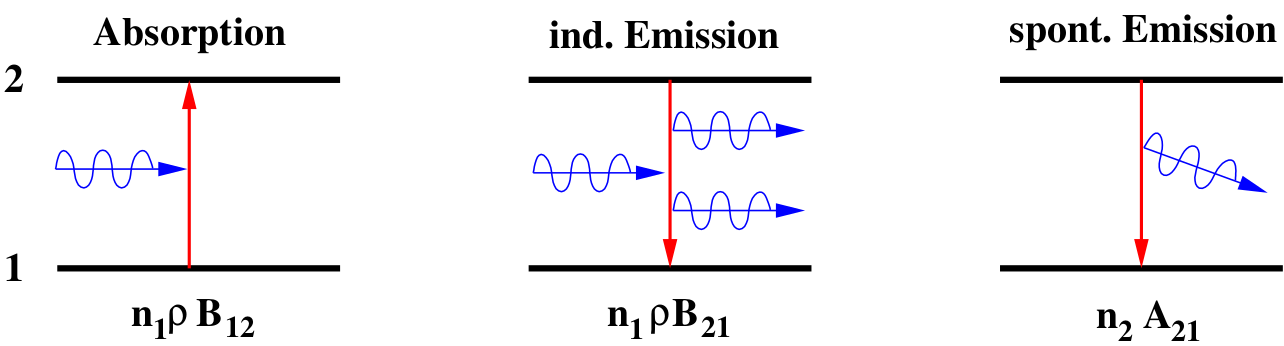
\includegraphics[ width= \textwidth]{pics/Emiss.png}
  \caption{Schematische Darstellung von Absorption und Emission eines Strahlungsfeldes 
\texorpdfstring{$\rho(\nu)$}{math} im Zwei-Niveau-System.}
  \label{fig:Emiss}
\end{figure}
\FloatBarrier
\paragraph{Der Resonator}
Die Verstärkung des Strahlungsfeldes nimmt exponentiell mit dem Laufweg im gepumpten Medium zu. 
Um die größtmögliche Verstärkung zu erhalten sollte der Laufweg möglichst groß gewählt sein, dafür wird 
ein Resonator verwendet. Der Resonator lässt den Laserstrahl das Medium mehrfach durchlaufen, dies wird 
durch zwei sich gegenüberstehenden Spiegeln, von den einer teildurchlässig ist, verwirklicht. 
Die Verlust durch die verwendeten Spiegel sollten möglichst gering sein, damit der Resonator mit Laserrohr 
einen Oszillator bildet. Besonders verlustarm sind konfokale Resonatoren, d.h. beide Spiegel sind 
sphärisch und im Fokus des jeweils anderem (Brennpunkte aufeinander). Ist die Verstärkung der induzierten 
Emission größer als die Verluste am Resonator, dann bildet das System ein selbstanregenden Oszillator 
und der Resonator wird als optisch stabil bezeichnet. Der optisch stabile Fall wird mit der Gleichung 
\begin{equation}
0 \leq g_1 \cdot g_2 < 1 
\label{eq:osF}
\end{equation}
beschrieben, dabei bezeichnen 
\begin{equation}
g_i = 1 - \frac{L}{r_i}	
\label{eq:gi}
\end{equation}
die Resonatorparameter der jeweiligen Resonatorspiegel. Die Resonatorparameter werden über die Gleichung 
\eqref{eq:gi}, die Krümmungsradien $r_i$ der Spiegel und der Resonatorlänge $L$ bestimmt.\\
Im Resonator bilden sich stehende Wellen aus, da es viele Frequenzen gibt, die die Resonanzbedingung im 
Resonator erfüllen. Die Anzahl $q$ der Wellenlängen die im Resonator die Resonanzbedingung erfüllen, wird 
longitudinale Mode genannt. Der Resonator kann aber auch in transversalen Moden schwingen, dies geschieht 
aufgrund von Unebenheiten oder Verkippung o.a. vom Spiegel. Die Moden des Resonators werden mit 
TEM$_{lpq}$ bezeichnet, dabei sind l und p die transversalen Modenzahlen und geben die Knoten in 
x- und y-Richtung an. Höhere Moden haben auch größere Verlust, weshalb der Resonator nur wenige 
transversale Moden isoliert und verstärkt. 
Eine Nährung für die Feldverteilung für konfokalen Resonator ist gegeben mit 
\flushleft
\begin{equation}
\begin{split}
E_{lpq} \propto \cos(l \phi) \frac{(2\rho)^2}{(1+Z^2)^{(1+l)/2}} 
\cdot L_p ^q\left(\frac{(2\rho)^2}{(1+Z^2)}\right)
\cdot \exp\left(-\frac{\rho^2}{(1+Z^2)}\right) \\
\cdot \exp\left( -i \left( \frac{(1+Z)\pi R}{\lambda} \frac{\rho^2 Z}{1 + Z^2} 
-(l+2\rho +1)\left(\frac{\pi}{2} - \symup{arctan}\left( \frac{1-Z}{1+Z} \right) \right) \right) \right) \\
\text{mit} \quad \rho = \left( \frac{2\pi}{R\lambda} \right)^{\frac{1}{2}} 
\quad \text{und} \quad Z = \frac{2z}{R} \; .
\end{split}
\label{eq:Elpq}
\end{equation}
Dabei bezeichnet $L_p ^q$ ein Laguerre-Polynom für Modenzahlen $p$ und $q$. Die Feldverteilung der jeweiligen 
Moden lassen sich über die ihre Intensitätsverteilung bestimmen $I \propto \lvert E_{lpq}^2 \rvert$. Die 
Mode mit der größten Intensität ist die TEM$_{000}$ Mode. Sie weist in transversaler Richtung keine 
Nullstelle auf. Die Intensität dieser Grundmode ist durch 
\begin{equation}
I(r) = I_0  \cdot \exp\left (\frac{-2r^2}{\omega^2} \right )	
\label{eq:IGM}
\end{equation}
gegeben, dabei bezeichnet $I_0$ die Maximalintensität, $r$ den Abstand zur optischen Achse und $2\omega$ den 
Strahldurchmesser. Der Radius des Strahls $\omega$ ist gegeben über 
\begin{equation}
\omega(z) = \omega_0 \sqrt{1+ \left( \frac{\theta z}{\omega_0} \right)^2}
\label{eq:SR}
\end{equation}
hier bezeichnet $z$ den Abstand zur minimalen Strahlentaille $\omega_0$ und 
$\theta = \frac{\lambda \omega_0}{\pi}$ die Strahldivergenz.
 
\begin{figure}
  \centering
  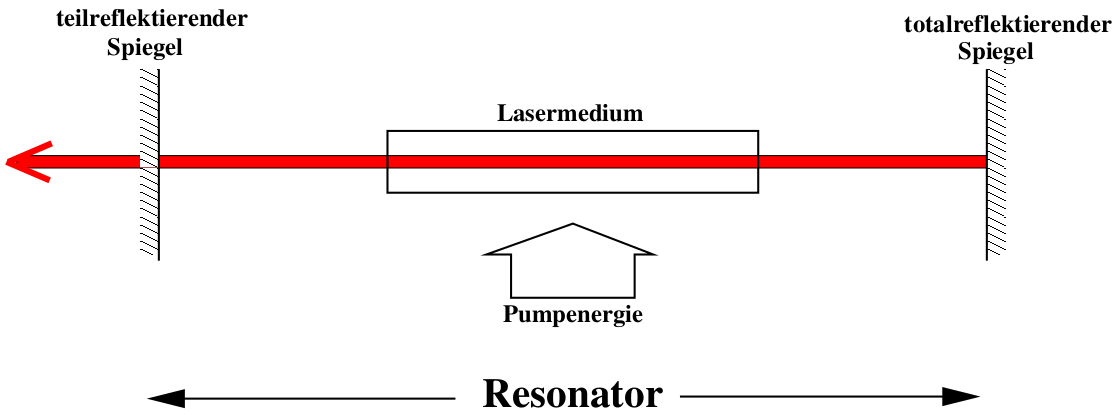
\includegraphics[height = 5cm]{pics/Resonator.png}
  \caption{Schematische Darstellung eines Lasers.}
  \label{fig:sl}
\end{figure}
\paragraph{Multimodenbetrieb}
Im Resonator bildet sich eine stehende Welle des Laserlichtes aus, auch Schwebung genannt. 
Dabei treten longitudinale Moden auf. Für Schwebungen gilt:
\begin{equation}
 N\cdot \frac{\lambda}{2} = L \quad \text{mit} \quad \lambda = \frac{\nu}{\symup{c}} \; .	
\label{eq:sw}
\end{equation}
Hier bezeichnet $\lambda$ die Wellenlänge des Lasers, $\nu$ die Frequenz und $\symup{c}$ die 
Lichtgeschwindigkeit. Daraus folgt
\begin{equation}
 \nu_N = \frac{\symup{c}}{2L}\cdot N \; ,
\end{equation}
das zeigt wie die Frequenz der entstehenden Moden abhängig von der Modenzahl $N$ ist. 
Aufgrund des Doppler-Effekts kann beobachtet werden, dass die Wellenlänge des Lasers nicht 
monochromatisch ist sondern gaußverteilt, um die Wellenlänge des induzierten Übergangs ist. 
Folglich gibt es mehrere Wellenlängen die für eine gegebene Resonatorlänge $L_i$ die Bedingung 
\eqref{eq:sw} erfüllen. Über die Knoten der Wellen die so, den Resonator verlassen, kann der 
Frequenzunterschied $\Delta \nu$ zwischen zwei Moden über 
\begin{equation}
\Delta \nu = \left .\frac{\symup{c}}{2L}  \right \rvert_{L_i}
\end{equation}
bestimmt werden. 
  
  
